% Copyright (C) 2009 Thomas L. Kula
% All Rights Reserved
%
% See the file LICENSE for license terms.
\documentclass[12pt]{article}
\usepackage{graphicx}
\usepackage{rotating}
\usepackage{fix-cm}
\setlength{\paperwidth}{5.5in}
\setlength{\paperheight}{8.5in}
\setlength{\textheight}{7.45in}
\setlength{\topmargin}{-1.0in}
\setlength{\oddsidemargin}{-0.5in}
\setlength{\evensidemargin}{-0.5in}
\setlength{\textwidth}{4.0in}
\setlength{\parindent}{0in}
\setlength{\parskip}{3mm}
\usepackage[print]{booklet} \nofiles
\source{\magstep0}{5.5in}{8.5in}
\target{\magstep0}{11in}{8.5in}
\setpdftargetpages
\pagestyle{empty}
\begin{document}


\begin{center}
{\fontsize{36}{48}\selectfont \textsc{Haiku a Day }}
\end{center}

\vspace*{3.5cm}

{\fontsize{26}{52}\selectfont 
From the sky it sinks
	 
A hard water that feels soft
	 
I look, it covers

}

\vspace*{5.0cm}
\begin{center}
{\large{Issue 54: December 2009}} \\[5mm]
{\fontsize{8}{8}\selectfont  \textsc{ St. Joshua Norton Press }} \\[1mm]
{\fontsize{6}{6}\selectfont Mathom House in Midtown \textbar The People's Republic of Ames }
\end{center}


\newpage

Remarkably, typing ``2010'' came fairly naturally. Much more quickly
than I would have expected.

--- Thomas

http://kula.tproa.net/had/ \\
kula@tproa.net

Download this and previous HADs at the website, so you can
print out your own (DIY, yeah!) or if you want me to send
you one, send me your address, and maybe a stamp if you
are feeling nice. Or send me something you've made ---
trades always appreciated, postcards are nice too.

\vspace*{2cm}

1 December 2009

Excitement brightens \\
And in its way lights the path \\
Pale in its guidance

2 December 2009

``I am become cake, \\
Tasty snack of tasty snacks \\
Look at me and nosh"

3 December 2009

The water swirling \\
Does not wash away my sins \\
Unless dishes count

\newpage

4 December 2009

In bringing order \\
There is chaos revealing \\
A crimp in the plans

5 December 2009

Standing twelve hours \\
Walking about, helping out \\
The Shadow Art Fair

6 December 2009

The day starts anew \\
I wonder where my shoes are \\
Oh, under the chair

7 December 2009

Under too much stress \\
It reacts with a loud snap \\
Making power safe

8 December 2009

Stuff high on a shelf \\
All self-inflicted {\em mathom} \\
No will to toss it

9 December 2009

Trite arithmatic \\
Making my brain curl up \\
Sums not adding up

10 December 2009

My old age revealed \\
Too much cheese upon my plate \\
A younger self weeps


\newpage

11 December 2009

A cold universe \\
Metal grinds eternally \\
Sweeping out the time

12 December 2009

Some simple errands \\
End up taking forever \\
Driving me insane

13 December 2009

Solitary leaf \\
Steadfast and not giving up \\
Winter does not sway

14 December 2009

Thinning to strengthen \\
A sinuous arc, deadly \\
At the edge force falls

15 December 2009

What is in this box, \\
And why do I still have it? \\
Less junk, my new goal

16 December 2009

From below the ground \\
You're torn, ground and made to stand \\
Gypsum, I salute!

17 December 2009

Detergent freezes \\
A fact that's useful to know \\
When it's cold outside


\newpage

18 December 2009

A gnawing pressure \\
Creeping, hiding, dark ichor \\
Jumps alive, ear ache

19 December 2009

Tea keeps me alive \\
That in such a simple gift \\
Should be that power

20 December 2009

The world becomes bright \\
And what was once elusive \\
Suddenly appears

21 December 2009

The morning hour \\
Appearing before it should \\
Awake before dawn

22 December 2009

Year's last day of work \\
Is not making me feel like \\
Doing anything

23 December 2009

Iowa below \\
Welcomes with a winter storm \\
Dancing in the sky

24 December 2009

Village full of life \\
Frozen in time, shrunk and still \\
Exist, fade, exist


\newpage

25 December 2009

The cutting cold wind \\
Causes haste going one way \\
Pause in the other

26 December 2009

Well the well's now well \\
From the dark depths come water \\
A mighty trickle

27 December 2009

A compact order \\
Piles become folded, packed \\
The airy grows dense

28 December 2009

I missed you, coffee! \\
Six days I've had but water \\
Slumping in my mug

29 December 2009

Organization \\
At least the promise of it \\
Fills me with much joy

30 December 2009

The cold settles in \\
Ready to stay, patiently \\
Waiting out its time

31 December 2009

Farewell to the aughts \\
I'm glad that I lived through them \\
When I'm an old man




\newpage

\begin{center}
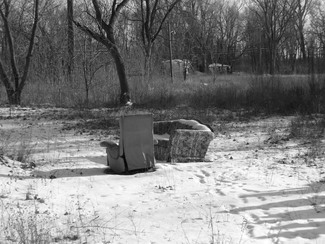
\includegraphics{water-street.jpg} \\[1cm]
Water Street Property Walk \\
{\tt http://kula.tproa.net/photos/2010/20100102-water-street/ }
\end{center}

\newpage

\thispagestyle{empty}
\vspace*{14cm}
\begin{sideways}
\Large{Thomas L. Kula}
\end{sideways}
\begin{sideways}
\Large{PO Box 980461}
\end{sideways}
\begin{sideways}
\Large{Ypsilanti MI 48198}
\end{sideways}


\end{document}


